\documentclass[tikz,convert={outfile=\jobname.svg}]{standalone}
%\usetikzlibrary{...}% tikz package already loaded by 'tikz' option
\usepackage{tikz-qtree}
\begin{document}
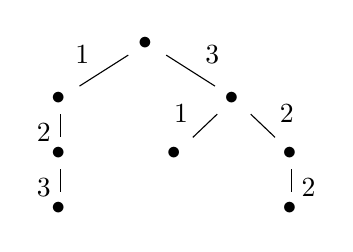
\begin{tikzpicture}[
    every tree node/.style={execute at begin node=\(\bullet\)},
    level distance=7mm,sibling distance=1cm,
    edge from parent path={(\tikzparentnode) -- (\tikzchildnode)}]
\Tree
[.\,
  \edge node[auto=right,pos=.6] {1};
  [.\,
    \edge node[auto=right,pos=.8] {2};
    [.\,
      \edge node[auto=right,pos=.8] {3};
      [.\,  ]
    ]
  ]
  \edge node[auto=left,pos=.6] {3};
  [.\,
    \edge node[auto=right,pos=.8] {1};
    [.\,  ]
    \edge node[auto=left,pos=.8] {2};
    [.\,
      \edge node[auto=left,pos=.8] {2};
      [.\,  ]
    ]
  ]
]
\end{tikzpicture}
\end{document}
